\apendice{Especificación de Requisitos}

\section{Introducción}
Este anexo recoge las necesidades funcionales que deberán ser soportadas por el sistema que va a ser desarrollado. Con el fin de obtener una buena documentación se deben identificar y describir los requisitos que debe el sistema satisfacer, pero sin entrar en cómo los va a resolver.

A día de hoy, no existe una autoridad que indique cómo se deben de realizar las especificaciones de requisitos \textit{software}, SRS. La comunidad se encuentra dividida entre <<la vieja escuela>> siguiendo guías de buenas prácticas (IEEE 830-1998~\cite{720574} ó 12207-2-2020~\cite{IEEE1220722020}), en contraposición con el \textit{Agile Manifiesto}, donde no se hace una especificación formal de toda la aplicación sino que cada 2-4 semanas se revisa y <<rehace>> en función de las necesidades del cliente.

Se va a realizar una combinación de ambos, por un lado se trabaja a lo largo del proyecto con una planificación ágil, y por otro se va a tener como referencia una especificación de requisitos que va a seguir la guía de buenas prácticas IEEE 830-1998. Ésta última recoge los siguientes puntos como referencias a una buena especificación de requisitos \textit{software}~\cite{ingenieriasoftwareytiemporeal_2020}.
\begin{itemize}
\item \textbf{Correcto.} Será correcto si, y sólo si, cada requisito declarado se encuentra en el \textit{software} entregado.
\item \textbf{Inequívoco.} Será inequívoco si, y solo si, cada requisitos declarado tiene sólo una interpretación. Cada característica de la última versión del producto se deberá describir con un único término.
\item \textbf{Completo.} Será completo si, y sólo si, incluye:
\begin{enumerate}
\item Los requisitos están relacionados a la funcionalidad, el desarrollo, las restricciones del diseño, los atributos y las interfaces externas. En particular debe reconocerse cualquier requisito externo impuesta por una especificación del sistema y debe tratarse.
\item La definición de las respuestas del \textit{software} a todos los posibles datos de la entrada del sistema y a toda clase de situaciones.
\item Tener todas las etiquetas llenas y referencias a todas las figuras, tablas, diagramas en el SRS y definición de todas las condiciones y unidades de medida.
\end{enumerate}
\item \textbf{Consistente.} Si un SRS <<choca>> con algún documento de nivel superior (~\textit{i.e.} una especificación de requisitos de sistema), entonces no será consistente.
\item \textbf{Comprobable.} Será comprobable si, y sólo si, cada requisito declarado es comprobable. A su vez un requisito será comprobable si, y sólo si, allí existe un proceso rentable finito con que una persona o la máquina puede verificar que el producto del \textit{software} reúne el requisito. Cualquier requisito ambiguo no es comprobable.
\item \textbf{Modificable}. Será modificable si, y sólo si, su estructura y estilo son tales que puede hacerse cualquier cambio a los requisitos fácilmente, completamente y de forma consistente mientras conserva la estructura y estilo.
\item \textbf{Identificable.} Será identificable si el origen de cada uno de los requisitos está claro y facilita de igual manera las referencias de cada requisito de desarrollo futuro o documentación del mismo.
\end{itemize}


\section{Objetivos generales}\label{objetivos-generales}
Los objetivos del proyecto se pueden separar en dos ramas.
\begin{enumerate}
\item Realización de un estudio de los métodos de selección de instancias más relevantes en la literatura y su aportación en problemas de aprendizaje Semi-Supervisado. Como producto final se desean tener dos bibliotecas con los principales algoritmos de selección de instancias y una de los principales algoritmos de aprendizaje Semi-Supervisado.
\item Integración de las bibliotecas anteriormente expuestas en la plataforma de MLaaS de la Universidad de Burgos (UBUMLaaS).
\item Rediseño completo de UBUMLaaS, modernización de la interfaz gráfica, de forma que sea más intuitivo su uso.
\item Nuevas funcionalidades para el usuario.
\item Administración integral del sistema a cargo del nuevo rol de administrador.
\end{enumerate}

En la biblioteca referida a los algoritmos de filtrado más comunes se implementarán algoritmos clásicos de la literatura como son CNN, RNN, ICF, ... Mientras que la biblioteca de algoritmos clásicos de Semi Supervisado contendrá \textit{Co-Training}, \textit{Tri-Training},\dots Estando estructuradas en forma de clases accesibles mediante importación clásica de paquetes. Deben de ser fácilmente escalables, posterior a la finalización del proyecto deben poder ampliarse sin añadir complejidad.

Las interfaces a diseñar se requieren que sean intuitivas, fáciles de entender y utilizar. Deberán de ser transparentes al usuario, impidiendo que este conozca la lógica de diseño de la aplicación, así como los posibles fallos internos que se puedan producir por acciones del sistema, del usuario, o de terceros.


\section{Usuarios del \textit{software}}\label{usuarios-participantes-software}
Cualquier persona podrá hacer uso de la aplicación UBUMLaaS, siendo únicamente necesarios una serie de datos básicos para su registro dentro de ella. 

Dentro de la aplicación se encuentra el usuario base y una generalización del mismo en forma de administrador. 
\begin{itemize}
\item \textbf{Usuario.} El usuario será el modelo base, en la forma de una persona la cual tendrá las capacidades de: crear experimentos y todas las funcionalidades asociadas con los mismos. Así como editar sus datos personales, añadir nuevos, quitar,\dots Y conocer sus estadísticas de uso de la última semana.

\item \textbf{Administrador.} Actor generalizado de usuario. Tiene todas las funcionalidades propias del usuario, pero además posee acceso a toda la parte de administración de la aplicación. En esta nueva parte posee acceso a la monitorización del sistema en tiempo real, a las estadísticas del mismo en cuanto a uso respecta, administración de todos los usuarios, etc. 
\end{itemize}

Un usuario es creado por una persona ajena que quiere registrarse en la aplicación, o por un administrador. Pero un administrador sólo puede ser <<creado>> (elevación de usuario a administrador) por otro administrador, y lo mismo para el caso contrario, pasar de administrador a usuario.


\section{Factores de riesgo}\label{factores-de-riesgo}
En esta sección se va a realizar un análisis de las `principales dificultades que se pueden encontrar a lo largo del desarrollo del proyecto \textit{software}. Mediante una identificación preventiva se podrá poner remedio a éstas de una manera más eficiente e impedir <<que vayan a más>>.

Se identifican los siguientes factores de riesgo:
\begin{enumerate}
\item \textbf{Desconocimiento teórico.} Se posee una cantidad muy limitada de conocimiento en la materia en la que el proyecto transcurre. El proyecto tiene un enfoque fuertemente relacionado con la minería de datos, un área hasta ahora inexplorada. El proyecto ya en su base más pura va a suponer un reto en el día a día.
\item \textbf{Documentación a utilizar.} Hasta ahora nunca se ha tratado con \textit{papers} o artículos científicos, mucho menos su lectura y comprensión, análisis y posterior implementación de los algoritmos propuestos. Puede suponer retrasos sin previo aviso un \textit{paper} con una alta complejidad, bien por la condensación de información, bien por la encapsulación de información, o simplemente por los conocimientos que se  requieren para entender el documento.
\item \textbf{Experiencia modificando un proyecto \textit{software}.} La experiencia personal dictamina que la modificación de proyectos que han sido iniciados por terceros (como se trabaja en la industria) conlleva una etapa de adaptación la cual no suele ser linear, sino exponencial, en función de la complejidad de la aplicación que se desea asimilar.
\item \textbf{Mínima experiencia con algunos lenguajes/bibliotecas.} El proyecto requiere del uso del lenguajes de programación como JavaScript, o lenguajes de marcas como son HTML, CSS, \LaTeX ... o bibliotecas como Flask o Vue. Con las que no se tiene prácticamente experiencia real de uso. Supondrá un esfuerzo extra e impedirá que determinadas tareas sean tan cortas como deberían serlo.
\item \textbf{Existencia del usuario final.} Se desconoce el usuario final de la aplicación, por lo que no se podrán realizar talleres, esto motivará a que el proyecto se creará como se cree que el usuario lo esperaría, pero sin su aprobación.
\item \textbf{Motivación del equipo de desarrollo.} En un proyecto nuevo y de este tipo, la experiencia personal es que antes o después habrá una pérdida de motivación para mantener un ritmo de trabajo óptimo.
\item \textbf{Compaginación con los estudios académicos. (Factor Tiempo).} El proyecto se desarrolla paralelamente al último curso de los estudios universitarios, debiendo ser correctamente compaginado para que <<nada pise a nada>> y no produzca retrasos. La escasez de tiempo puede suponer un problema en caso de que en los primeros \textit{sprints} de trabajo no se alcance un ritmo de desarrollo adecuado, la fecha límite es conocida desde el inicio del proyecto y se debe de tener en cuenta.
\item \textbf{Corrupción del alcance.} En caso de que los objetivos del proyecto no estén claramente definidos. Una correcta hoja de ruta permitirá a todos los involucrados a conocer la parametrización deseada. Estando muy relacionado con la motivación (no <<ver el final>> del proyecto nunca) y por consecuencia con el ritmo de trabajo.
\item \textbf{Coste de la infraestructura.} Se debe tener en cuenta que se va a desarrollar una aplicación web, pero por su naturaleza necesitará un servidor (distribuido o no) para su ejecución. A baja escala puede no ser un riesgo, pero se debe vigilar en caso de despliegue en las principales \textit{cloud}.
\item \textbf{Falta de claridad.} La comunicación entre todas las partes implicadas debe de ser lo más fluida y natural posible, permitiendo minimizar los retrasos por tener que rehacer algo que se había especificado de una forma y no se había entendido correctamente (Inequívoco).
\end{enumerate}

\section{Catálogo de requisitos}\label{catalogo-de-riquisitos}
En esta sección se van a definir de forma clara, completa, precisa y verificable todas las funcionalidades y restricciones del sistema.

A pesar de que el proyecto tiene dos <<enfoques>>, la parte de UBUMLaaS y la parte de bibliotecas, los requisitos funcionales y no funcionales se van a desglosar juntos, siguiendo el orden en el que aparecen en este texto.

\subsection{Requisitos funcionales}\label{requisitos-funcionales}
\begin{itemize}
\tightlist
\item
  \textbf{RF-1 Uso de algoritmos de aprendizaje automático.} La aplicación debe de ser capaz de entrenar un modelo entrenado con un algoritmo elegido por el usuario y posteriormente utilizar dicho modelo para predecir sobre un conjunto de datos.

\begin{itemize}
\tightlist
\item \textbf{RF-1.1 Entrenar el modelo.} El usuario debe de poder entrenar un modelo nuevo en cada experimento.
    \begin{itemize}
    \tightlist
    \item \textbf{RF-1.1.1 Elección del algoritmo.} El usuario debe de ser capaz de elegir el algoritmo que considere oportuno de entre todos los posibles.
     \item \textbf{RF-1.1.2 Parametrización del algoritmo.} El usuario debe poder parametrizar el algoritmo cómo considere oportuno para su problema.
     \item \textbf{RF-1.1.3 Conjuntos de datos especiales.} El usuario en caso de realizar experimentos de Semi-Supervisado tendrá que utilizar conjuntos de datos preparados para ello.
    \end{itemize}
    \item \textbf{RF-1.2 Descarga del modelo.} El usuario debe de ser capaz de descargar el modelo para poder usarlo en otros sistemas.
    \item \textbf{RF-1.3 Reutilización del modelo.} El usuario debe de ser capaz de crear un modelo  utilizando una parametrización base de otro modelo existente en el sistema.
    \item \textbf{RF-1.4 Predicción de nuevos prototipos.} El usuario debe de ser capaz de utilizar un modelo ya entrenado para predecir nuevos conjuntos de datos que posean la misma relación de atributos.
    \item \textbf{RF-1.5 Estadísticas del entrenamiento.} El usuario debe de ser capaz de visualizar las estadísticas del experimento ejecutado, independientemente de si el entrenamiento ha sido mediante validación cruzada o con partición mediante porcentajes para entrenamiento y pruebas.
	\item \textbf{RF-1.6 Consulta de experimentos.} El usuario debe de poder consultar aquellos experimentos que ha lanzado.
  \end{itemize}
\item \textbf{RF-2 Uso de algoritmos de selección de instancias.} El usuario deberá poder elegir si usar o no, para cualquier experimento independientemente de su naturaleza, los algoritmos de selección de instancias codificados.
	\begin{itemize}
	\tightlist
	\item \textbf{RF-2.1 Parametrización del algoritmo.} El usuario debe poder parametrizar el algoritmo cómo considere oportuno para su problema.
\end{itemize}
\item \textbf{RF-3 Administración de usuarios.}
	\begin{itemize}
	\tightlist
	\item \textbf{RF-3.1 Dar de alta nuevos usuarios.} El administrador debe poder crear un nuevo usuario con la información básica.
	\begin{itemize}
	\tightlist
	\item \textbf{RF-3.1.1 Activación del usuario.} El sistema debe mandar el correspondiente correo de activación al nuevo usuario.
	\item \textbf{RF-3.1.2 Contraseña del usuario.} Se generará una contraseña complaciente con la política de seguridad de la plataforma. En ningún momento dicha contraseña podrá ser conocida por ningún administrador o miembro del sistema. El usuario deberá de restaurar la contraseña antes de iniciar sesión por primera vez.
	\end{itemize}
	\item \textbf{RF-3.2 Activación de usuarios.} El administrador debe de poder activar o desactivar a un usuario en concreto.
	\item \textbf{RF-3.3 Hacer administrador a un usuario.} El administrador debe de poder hacer nuevos usuarios administradores.
	\item \textbf{RF-3.4 Eliminar a un usuario.} El administrador debe de poder eliminar a un usuario cualquiera del sistema, independientemente de si este usuario es administrador o no.
	\item \textbf{RF-3.5 Auto-Modificación del administrador.} El administrador no debe de poder desactivarse, quitarse de administrador o eliminarse a sí mismo.
	\end{itemize}
\item \textbf{RF-4 Modificación de datos del usuario.}
	\begin{itemize}
	\tightlist
	\item \textbf{RF-4.1 Datos básicos.} El usuario debe de poder modificar sus datos básicos, pero nunca pudiendo dejarlos <<en blanco>>.
	\item \textbf{RF-4.2 Datos adicionales.} El usuario debe de poder añadir, modificar o eliminar, una serie de datos adicionales.
	\item \textbf{RF.4.3 Imagen de perfil.} El usuario debe de poder actualizar su foto de perfil, cumpliendo con una serie de requisitos de tamaño y formato.
	\item \textbf{RF-4.4 Actualización de contraseña.} El usuario deberá de poder actualizar su contraseña en caso de considerarlo necesario.
	\end{itemize}
	\pagebreak
\item \textbf{RF-5 Administración del sistema en tiempo real.}
	\begin{itemize}
	\tightlist
	\item \textbf{RF-5.1 Información de red.} El administrador debe de poder visualizar la configuración actual de red en la que la plataforma está desplegada.
	\item \textbf{RF-5.2 Información de carga.} El administrador debe de poder visualizar la carga del actual del sistema en términos de uso de procesador y memoria.
	\item \textbf{RF-5.3 Información adicional.} El administrador debe de poder visualizar datos adicionales como el uso de red, almacenamiento disponible, \dots
	\end{itemize}
\item \textbf{RF-6 Estadísticas de uso.}
	\begin{itemize}
	\tightlist
	\item \textbf{RF-6.1 Estadísticas de uso para usuarios.}
	\begin{itemize}
	\tightlist
		\item \textbf{RF-6.1.1 Uso últimos 7 días.} El usuario debe de poder visualizar unas estadísticas generales de su uso particular en los últimos 7 días naturales.
		\item \textbf{RF-6.1.2 Uso de cada tipo de algoritmo.} El usuario debe de poder visualizar qué y cuántos algoritmos de cada tipo ha ejecutado. Además del tiempo de ejecución global de cada tipo.
		\item \textbf{RF-6.1.3 Estadísticas generales.} El usuario debe de poder conocer cuántos experimentos ha ejecutado en total y cuántos conjuntos de datos tiene alojados en el sistema.
	\end{itemize}
	\item \textbf{RF-6.2 Estadísticas de uso para administradores.}
	\begin{itemize}
		\item \textbf{RF-6.2.1 Estadísticas generales}. El administrador debe de poder de un vistazo conocer el uso general que se le está dando al sistema. (Número de experimentos, número de usuarios, tipo de experimentos,\dots)
		\item \textbf{RF-6.2.2 Uso últimos 7 días.} El administrador debe de poder conocer el número de experimentos que se han ejecutado cada día de los últimos 7 días naturales.
		\item \textbf{RF-6.2.3 Distribución de los usuarios.} El administrador debe de poder conocer las estadísticas generales de uso y países de origen de los usuarios del sistema.
	\end{itemize}
	\end{itemize}
\end{itemize}
\pagebreak
\subsection{Requisitos no funcionales}\label{requisitos-no-funcionales}
\begin{itemize}
\item \textbf{RNF-1 Usabilidad.} La plataforma debe de ser fácil tanto de aprender a utilizar como clara a la hora de reportar los errores que se puedan cometer. La interfaz debe ser intuitiva.
\item \textbf{RNF-2 Rendimiento.} La interfaz web no se puede quedar <<colgada>>, además debe de tener unos tiempos de carga razonables.
\item \textbf{RNF-3 Escalabilidad.} La plataforma debe soportar que se le añadan nuevas funcionalidades con relativa facilidad.
\item \textbf{RNF-4 Disponibilidad.} La plataforma debe de ser accesible a través de Internet sin importar la geolocalización del cliente.
\item \textbf{RNF-5 Fiabilidad.} La plataforma debe de garantizar que los modelos calculados son precisos. Además de en caso de pérdidas de conexión, que no ocurran peérdidas de datos.
\item \textbf{RNF-6 Seguridad.} La plataforma debe gestionar correctamente \textit{tokens}, contraseñas, así como el control de administradores o no.
\item \textbf{RNF-7 Mantenibilidad.} La plataforma debe cumplir los estándares de código de cada uno de los lenguajes en los que se desarrolla. 
\item \textbf{RNF-8 Soporte.} La plataforma debe dar soporte a ficheros CSV y ARFF como mínimo. Así como ser compatible con HTML5.
\item \textbf{RNF-9 Monitorización.} La plataforma debe ser fácilmente monitorizable por un administrador.
\item \textbf{RNF-10 Internacionalización.} La plataforma debe de estar desarrollada en un inglés sencillo y fácil de comprender por todo tipo de usuarios no nativos.
\item \textbf{RNF-11 Respuesta autónoma.} En caso de inicio o reinicio, el tiempo empleado por la plataforma hasta estar al 100\% de operatibilidad de nuevo debe ser inferior a los 3 minutos.
\end{itemize}
\newpage
\section{Especificación de requisitos}

Dentro de esta sección se desarrolla el Diagrama de Casos de Uso, ver Figura~\ref{img:diagrama-casos-uso}, y la explicación correspondiente de cada uno de ellos.

\begin{figure}[h!]
	\centering
	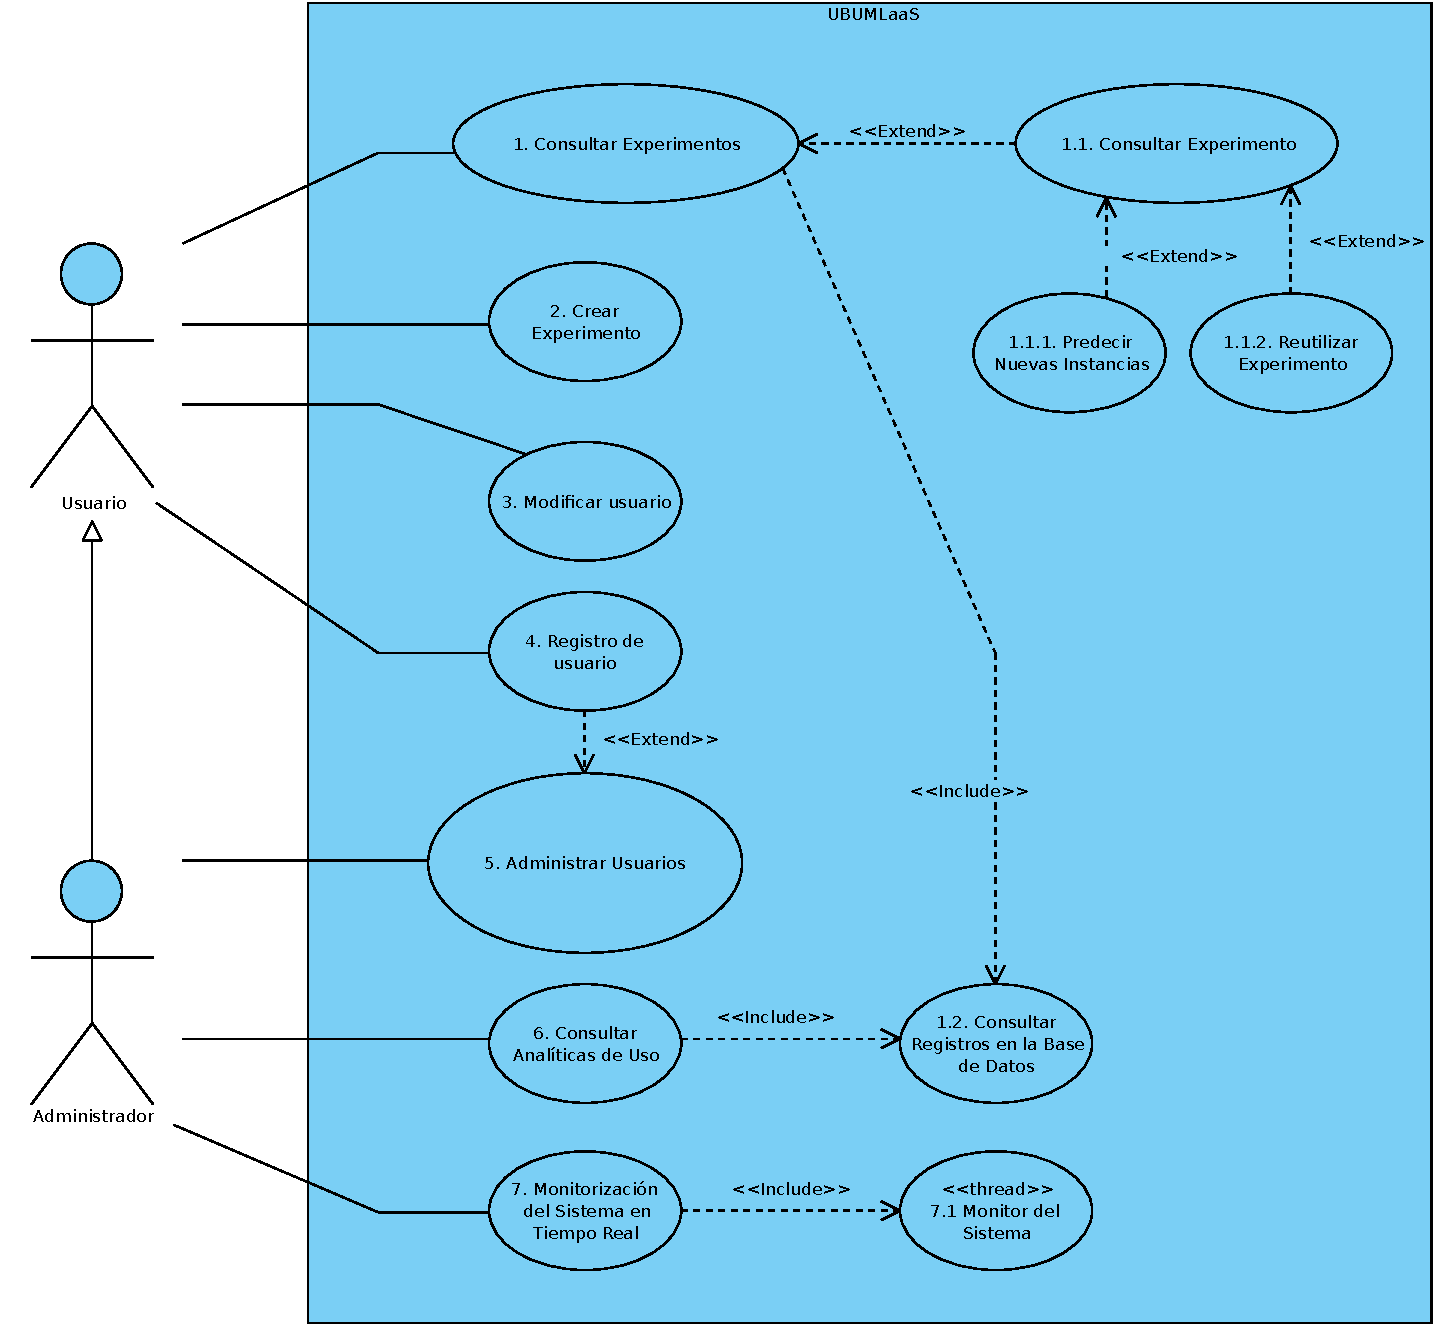
\includegraphics[scale=0.5]{../img/anexos/requisitos/Casos-de-uso}
	\caption{Diagrama de casos de uso.}\label{img:diagrama-casos-uso}
\end{figure}

\subsection{Actores}
Actuarán dos actores con el sistema, un usuario (el actor general) y un administrador (actor especializado heredado del usuario).

\subsection{Casos de uso}\label{casos-de-uso}
A continuación se detallan las tablas correspondientes a los casos de uso anteriormente planteados, en orden.

% Caso de Uso 1 -> Consultar Experimentos.
\begin{table}[p]
\centering
\begin{tabularx}{\linewidth}{ p{0.21\columnwidth} p{0.71\columnwidth} }
\toprule
\textbf{CU-1} & \textbf{Consultar Experimentos}\\
\toprule
\textbf{Versión} & 1.0\\
\textbf{Autor} & Daniel Puente Ramírez\\
\textbf{Requisitos asociados} & RF-1.3, RF-1.5, RF-1.6\\
\textbf{Descripción} & Permite al usuario consultar sus experimentos y reutilizarlos.\\
\textbf{Precondición} & El sistema de colas se encuentra en ejecución.\\
\textbf{Acciones} &
\begin{enumerate}
\def\labelenumi{\arabic{enumi}.}
\tightlist
\item El usuario entra en la plataforma.
\item Hace \textit{click} en <<Mis Experimentos>>.
\item Por cada experimento lanzado se da la opción de ver detalle, reutilizar o eliminar.
\end{enumerate}\\
\textbf{Postcondición} & El número de experimentos mostrados al usuario es igual al número de experimentos asociados con ese ID en la base de datos.\\
\textbf{Excepciones} & No existen excepciones posibles.\\
\textbf{Importancia} & Alta \\
\bottomrule
\end{tabularx}
\caption{CU-1 Consultar Experimentos.}
\end{table}

% Caso de Uso 1.1 -> Consultar Experimento
\begin{table}[p]
\centering
\begin{tabularx}{\linewidth}{ p{0.21\columnwidth} p{0.71\columnwidth} }
\toprule
\textbf{CU-1.1} & \textbf{Consultar Experimento}\\
\toprule
\textbf{Versión} & 1.0\\
\textbf{Autor} & Daniel Puente Ramírez\\
\textbf{Requisitos asociados} & RF-1.2, RF-1.3, RF-1.4, RF-1.5\\
\textbf{Descripción} & Permite al usuario consultar un experimento en concreto, si ha finalizado, junto con las métricas reportadas.\\
\textbf{Precondiciones} & 
\begin{itemize}
\tightlist
\item El experimento existe.
\item En caso de haber finalizado y tener métricas de rendimiento, se cargan.
\end{itemize}\\
\textbf{Acciones} &
\begin{enumerate}
\def\labelenumi{\arabic{enumi}.}
\tightlist
\item El usuario entra en la plataforma.
\item Hace \textit{click} en <<Mis Experimentos>>.
\item Por cada experimento lanzado se da la opción de ver detalle, reutilizar o eliminar.
\item Dentro de ver en detalle puede predecir nuevas instancias o descargar el modelo, así como consultar las métricas resultantes. En caso de haber fallado se muestra el motivo del fallo.
\end{enumerate}\\
\textbf{Postcondición} & El identificador del experimento no varía independientemente de lo que el usuario haga con él.\\
\textbf{Excepciones} & No existen excepciones posibles.\\
\textbf{Importancia} & Media \\
\bottomrule
\end{tabularx}
\caption{CU-1.1 Consultar Experimento.}
\end{table}


% Caso de Uso 1.1.1 -> Predecir Nuevas Instancias
\begin{table}[p]
\centering
\begin{tabularx}{\linewidth}{ p{0.21\columnwidth} p{0.71\columnwidth} }
\toprule
\textbf{CU-1.1.1} & \textbf{Predecir Nuevas Instancias}\\
\toprule
\textbf{Versión} & 1.0\\
\textbf{Autor} & Daniel Puente Ramírez\\
\textbf{Requisitos asociados} & RF-1.4\\
\textbf{Descripción} & Permite al usuario predecir nuevas instancias en función a un modelo previamente entrenado.\\
\textbf{Precondiciones} & 
\begin{itemize}
\tightlist
\item El experimento existe y ha finalizado.
\item Las nuevas instancias a predecir tienen los mismos atributos que con las que se entrenó el modelo.
\end{itemize}\\
\textbf{Acciones} &
\begin{enumerate}
\def\labelenumi{\arabic{enumi}.}
\tightlist
\item El usuario entra en la plataforma.
\item Hace \textit{click} en <<Mis Experimentos>>.
\item Por cada experimento lanzado se da la opción de ver detalle, reutilizar o eliminar.
\item Dentro de ver en detalle hace \textit{click} en <<Predict>>.
\item Sube el conjunto de datos a predecir.
\item Se le muestra al usuario el resultado de la predicción.
\end{enumerate}\\
\textbf{Postcondición} & El modelo no se ha visto afectado por el proceso de predicción.\\
\textbf{Excepciones} & El conjunto de datos pasado no cumple con los requisitos para el modelo.\\
\textbf{Importancia} & Alta \\
\bottomrule
\end{tabularx}
\caption{CU-1.1.1 Predecir Nuevas Instancias.}
\end{table}


% Caso de Uso 1.1.2 -> Reutilizar Experimento
\begin{table}[p]
\centering
\begin{tabularx}{\linewidth}{ p{0.21\columnwidth} p{0.71\columnwidth} }
\toprule
\textbf{CU-1.1.2} & \textbf{Reutilizar Experimento}\\
\toprule
\textbf{Versión} & 1.0\\
\textbf{Autor} & Daniel Puente Ramírez\\
\textbf{Requisitos asociados} & RF-1, RF-1.1, RF-1.1.1, RF-1.1.2, RF-1.1.3, RF-1.3\\
\textbf{Descripción} & Permite al usuario reutilizar el experimento que ya había creado.\\
\textbf{Precondición} & El experimento base existe.\\
\textbf{Acciones} &
\begin{enumerate}
\def\labelenumi{\arabic{enumi}.}
\tightlist
\item El usuario entra en la plataforma.
\item Hace \textit{click} en <<Mis Experimentos>>.
\item Busca el experimento del que desea obtener la parametrización para uno nuevo.
\item Hace \textit{click} en <<Reuse>>.
\end{enumerate}\\
\textbf{Postcondiciones} & 
\begin{enumerate}
\tightlist
\item El modelo base no se ha visto afectado.
\item El usuario se encuentra en la pantalla <<Nuevo Experimento>> con la configuración <<nueva>>.
\end{enumerate}\\
\textbf{Excepciones} & 
\begin{itemize}
\tightlist
\item Algún parámetro interno ha cambiado y ya no se puede reutilizar el experimento.
\item Solo se puede recuperar parte de la configuración.
\end{itemize}\\
\textbf{Importancia} & Media \\
\bottomrule
\end{tabularx}
\caption{CU-1.1.2 Reutilizar Experimento.}
\end{table}

% Caso de Uso 1.2 -> Consultar Registros en la Base de Datos
\begin{table}[p]
\centering
\begin{tabularx}{\linewidth}{ p{0.21\columnwidth} p{0.71\columnwidth} }
\toprule
\textbf{CU-1.2} & \textbf{Consultar Registros en la Base de Datos}\\
\toprule
\textbf{Versión} & 1.0\\
\textbf{Autor} & Daniel Puente Ramírez\\
\textbf{Requisitos asociados} & RF-1, RF-2, RF-3, RF-4, RF-5, RF-6\\
\textbf{Descripción} & Recuperación de los registros necesarios de la base de datos.\\
\textbf{Precondición} & Existen los registros.\\
\textbf{Acciones} &
\begin{enumerate}
\def\labelenumi{\arabic{enumi}.}
\tightlist
\item El usuario entra en la plataforma.
\item Realiza alguna acción relacionada con la base de datos.
\item Se le devuelven los datos solicitados, y/o
\item Se almacenan los nuevos datos.
\end{enumerate}\\
\textbf{Postcondición} & La integridad de la base de datos no se ha visto afectada.\\
\textbf{Excepciones} & Intento de escritura simultánea por parte de dos usuarios.\\
\textbf{Importancia} & Alta \\
\bottomrule
\end{tabularx}
\caption{CU-1.2 Consultar Registros en la Base de Datos.}
\end{table}

% Caso de Uso 2 -> Crear Experimento
\begin{table}[p]
\centering
\begin{tabularx}{\linewidth}{ p{0.21\columnwidth} p{0.71\columnwidth} }
\toprule
\textbf{CU-2} & \textbf{Crear Experimento}\\
\toprule
\textbf{Versión} & 1.0\\
\textbf{Autor} & Daniel Puente Ramírez\\
\textbf{Requisitos asociados} & RF-1, RF-1.1, RF-1.1.1, RF-1.1.2, RF-1.1.3, RF-2, RF-2.1\\
\textbf{Descripción} & Permite al usuario crear un nuevo experimento.\\
\textbf{Precondición} & La parametrización es correcta.\\
\textbf{Acciones} &
\begin{enumerate}
\def\labelenumi{\arabic{enumi}.}
\tightlist
\item El usuario entra en la plataforma.
\item Hace \textit{click} en <<Nuevo Experimento>>.
\item Rellena el formulario en función de un conjunto de datos y una técnica de aprendizaje automático.
\item Hace \textit{click} en <<Crear>>.
\end{enumerate}\\
\textbf{Postcondiciones} & 
\begin{enumerate}
\tightlist
\item El experimento ha sido añadido a las colas de ejecución.
\item El usuario recibe un correo electrónico con la finalización del experimento.
\end{enumerate}\\
\textbf{Excepciones} & El experimento ha sido incorrectamente parametrizado y se ha levantado una excepción al intentar ejecutarlo.\\
\textbf{Importancia} & Alta \\
\bottomrule
\end{tabularx}
\caption{CU-2 Crear Experimento.}
\end{table}

% Caso de Uso 3 -> Modificar Usuario
\begin{table}[p]
\centering
\begin{tabularx}{\linewidth}{ p{0.21\columnwidth} p{0.71\columnwidth} }
\toprule
\textbf{CU-3} & \textbf{Modificar Usuario}\\
\toprule
\textbf{Versión} & 1.0\\
\textbf{Autor} & Daniel Puente Ramírez\\
\textbf{Requisitos asociados} & RF-4, RF-4.1, RF-4.2, RF-4.3, RF-4.4\\
\textbf{Descripción} & Permite al usuario modificar sus datos personales dentro de la plataforma.\\
\textbf{Precondición} & Los datos del usuarios son recuperados de la base de datos.\\
\textbf{Acciones} &
\begin{enumerate}
\def\labelenumi{\arabic{enumi}.}
\tightlist
\item El usuario entra en la plataforma.
\item Hace \textit{click} en <<Mis Experimentos>>.
\item Hace \textit{click} en <<Editar Perfil>>.
\item Modifica los datos como considere oportuno.
\item Hace \textit{click} en <<Guardar>>.
\end{enumerate}\\
\textbf{Postcondiciones} & 
\begin{enumerate}
\tightlist
\item Todos los campos son validados de forma que individualmente cumplan sus respectivas restricciones de formato.
\item Para aquellos campos que deben ser únicos, se garantiza su unicidad.
\item Los datos actualizados son visibles desde el momento en el que se actualiza la página para el usuario.
\end{enumerate}\\
\textbf{Excepciones} & Modificación concurrente de la base de datos.\\
\textbf{Importancia} & Baja \\
\bottomrule
\end{tabularx}
\caption{CU-3 Modificar Usuario.}
\end{table}

% Caso de Uso 4 -> Registro de Usuario
\begin{table}[p]
\centering
\begin{tabularx}{\linewidth}{ p{0.21\columnwidth} p{0.71\columnwidth} }
\toprule
\textbf{CU-4} & \textbf{Registro de Usuario}\\
\toprule
\textbf{Versión} & 1.0\\
\textbf{Autor} & Daniel Puente Ramírez\\
\textbf{Requisitos asociados} & RF-3, RF-3.1, RF-3.1.1, RF-3.1.2\\
\textbf{Descripción} & Permite al administrador crear un nuevo usuario, o a un cliente registrarse en la plataforma y convertirse en administrador.\\
\textbf{Precondiciones} & No existen precondiciones.\\
\textbf{Acciones} &
\begin{enumerate}
\def\labelenumi{\arabic{enumi}.}
\tightlist
\item El administrador entra en la plataforma.
\item Hace \textit{click} en <<Usuarios>> en el panel lateral de administración.
\item Hace \textit{click} en <<Nuevo Usuario>>.
\item Introduce los datos del nuevo usuario.
\item Hace \textit{click} en <<Guardar>>.
\end{enumerate}\\
\textbf{Postcondiciones} & 
\begin{enumerate}
\tightlist
\item Todos los campos son validados de forma que individualmente cumplan sus respectivas restricciones de formato.
\item Para aquellos campos que deben ser únicos, se garantiza su unicidad.
\item El nuevo usuario recibe un correo electrónico con el \textit{token} de activación de la cuenta.
\end{enumerate}\\
\textbf{Excepciones} & Modificación concurrente en la base de datos.\\
\textbf{Importancia} & Baja \\
\bottomrule
\end{tabularx}
\caption{CU-4 Registro de Usuario.}
\end{table}

% Caso de Uso 5 -> Administrar Usuarios
\begin{table}[p]
\centering
\begin{tabularx}{\linewidth}{ p{0.21\columnwidth} p{0.71\columnwidth} }
\toprule
\textbf{CU-5} & \textbf{Administrar Usuarios}\\
\toprule
\textbf{Versión} & 1.0\\
\textbf{Autor} & Daniel Puente Ramírez\\
\textbf{Requisitos asociados} & RF-3, RF-3.1, RF-3.1.1, RF-3.1.2, RF-3.2, RF-3.3, RF-3.4, RF-3.5\\
\textbf{Descripción} & Permite al administrador crear, (de)activar, hacer (o quitar de) administrador, o eliminar a un usuario.\\
\textbf{Precondición} & El usuario a modificar no es el mismo usuario que está modificando.\\
\textbf{Acciones} &
\begin{enumerate}
\def\labelenumi{\arabic{enumi}.}
\tightlist
\item El administrador entra en la plataforma.
\item Hace \textit{click} en <<Usuarios>> en el panel lateral de administración.
\item Puede buscar si así lo desea al usuario en cuestión.
\item Realiza las modificaciones pertinentes.
\end{enumerate}\\
\textbf{Postcondición} & La modificación ha sido correcta.\\
\textbf{Excepciones} & Modificación concurrente en la base de datos.\\
\textbf{Importancia} & Media \\
\bottomrule
\end{tabularx}
\caption{CU-5 Administrar Usuarios.}
\end{table}

% Caso de Uso 6 -> Consultar Analíticas de Uso
\begin{table}[p]
\centering
\begin{tabularx}{\linewidth}{ p{0.21\columnwidth} p{0.71\columnwidth} }
\toprule
\textbf{CU-6} & \textbf{Consultar Analíticas de Uso}\\
\toprule
\textbf{Versión} & 1.0\\
\textbf{Autor} & Daniel Puente Ramírez\\
\textbf{Requisitos asociados} & RF-6, RF-6.1, RF-6.1.1, RF-6.1.2, RF-6.1.3, RF-6.2, RF-6.2.1, RF-6.2.2, RF-6.2.3\\
\textbf{Descripción} & Permite a un usuario comprobar sus estadísticas de uso. Y si es administrador, las del la plataforma.\\
\textbf{Precondición} & Existen estadísticas que mostrar.\\
\textbf{Acciones} (para el usuario) &
\begin{enumerate}
\def\labelenumi{\arabic{enumi}.}
\tightlist
\item El usuario entra en la plataforma.
\item Hace \textit{click} en <<Mis Experimentos>>.
\item Hace \textit{click} en <<Estadísticas>>.
\item Puede visualizar las estadísticas generales de la plataforma.
\end{enumerate}\\
\textbf{Acciones} (para el administrador) &
\begin{enumerate}
\def\labelenumi{\arabic{enumi}.}
\tightlist
\item El administrador entra en la plataforma.
\item Hace \textit{click} en \textit{<<Dashboard>>} en el panel lateral de administración.
\item Puede visualizar las estadísticas generales de la plataforma.
\end{enumerate}\\
\textbf{Postcondiciones} & No existen postcondiciones.\\
\textbf{Excepciones} & No existen excepciones.\\
\textbf{Importancia} & Alta \\
\bottomrule
\end{tabularx}
\caption{CU-6 Consultar Analíticas de Uso.}
\end{table}

% Caso de Uso 7 -> Monitorización del Sistema en Tiempo Real
\begin{table}[p]
\centering
\begin{tabularx}{\linewidth}{ p{0.21\columnwidth} p{0.71\columnwidth} }
\toprule
\textbf{CU-7} & \textbf{Monitorización del Sistema en Tiempo Real}\\
\toprule
\textbf{Versión} & 1.0\\
\textbf{Autor} & Daniel Puente Ramírez\\
\textbf{Requisitos asociados} & RF-5, RF-5.1, RF-5.2, RF-5.3\\
\textbf{Descripción} & Permite al administrador comprobar el estado de carga actual del sistema.\\
\textbf{Precondición} & Existen registros de datos para calcular las estadísticas que mostrar.\\
\textbf{Acciones} &
\begin{enumerate}
\def\labelenumi{\arabic{enumi}.}
\tightlist
\item El administrador entra en la plataforma.
\item Hace \textit{click} en \textit{<<Live Monitor>>} en el panel lateral de administración.
\item Puede visualizar las estadísticas generales de la plataforma.
\end{enumerate}\\
\textbf{Postcondiciones} & No existen postcondiciones.\\
\textbf{Excepción} & En caso de que no existan datos aún.\\
\textbf{Importancia} & Alta \\
\bottomrule
\end{tabularx}
\caption{CU-7 Monitorización del Sistema en Tiempo Real.}
\end{table}

% Caso de Uso 7.1 -> Monitor del Sitema
\begin{table}[p]
\centering
\begin{tabularx}{\linewidth}{ p{0.21\columnwidth} p{0.71\columnwidth} }
\toprule
\textbf{CU-7.1} & \textbf{Monitor del Sistema}\\
\toprule
\textbf{Versión} & 1.0\\
\textbf{Autor} & Daniel Puente Ramírez\\
\textbf{Requisitos asociados} & RF-5.1, RF-5.2, RF-5.3\\
\textbf{Descripción} & Proceso de recolección de información de uso del sistema.\\
\textbf{Precondición} & Glances está instalado en el sistema.\\
\textbf{Acciones} & Ninguna, ejecución en paralelo en el sistema.\\
\textbf{Postcondiciones} & No existen postcondiciones.\\
\textbf{Excepción} & No existen excepciones.\\
\textbf{Importancia} & Alta \\
\bottomrule
\end{tabularx}
\caption{CU-7.1 Monitor del Sistema.}
\end{table}
